\documentclass[11pt]{article}
\usepackage{graphicx}
\graphicspath{ {./images/} }

\usepackage{algorithm}
\usepackage{algpseudocode}
\usepackage{hyperref}

\usepackage{sectsty}
\usepackage{graphicx}
\usepackage[font=small,labelfont=bf]{caption} % Required for specifying captions to tables and figures

% Margins
\topmargin=-0.45in
\evensidemargin=0in
\oddsidemargin=0in
\textwidth=6.5in
\textheight=9.0in
\headsep=0.25in

\title{ %

\includegraphics[width=0.4\textwidth]{UniCT-Logo-Nero}~\\
A solution for MWVC using Iterated Local Search \\ 
\large Laboratorio Intelligenza Artificiale (LM-18) \\ Università degli Studi di Catania - A.A 2021/2022 \\
}
\author{ Danilo Leocata \\ Docente: Mario Pavone}
\date{\today}

\begin{document}

\maketitle	
\pagebreak

% Optional TOC
% \tableofcontents
% \pagebreak

%--Paper--

\section{Introduzione}

Si propone una soluzione per il Weight Vertex Cover problem utilizzando l'Iterated Local Search: l'obbiettivo proposto è trovare la migliore soluzione, data un istanza, con il minimo numero di iterazioni. I
Il codice è stato interamente implementato in Java senza l'utilizzo librerie esterne eccetto \verb|matplotlib4j| per la generazione dei grafici di convergenza e \verb|CSVWriter| per la generazione del \verb|.csv| dei ottenuti (non sono stati caricati tutti per evitare di appesantire troppo la repository).

Il codice è interamente disponibile al seguente repository GitHub \href{https://github.com/khalld/mwvc-using-ils-java}{https://github.com/khalld/mwvc-using-ils-java}, nel quale sono stati caricati i risultati di benchmark e parte dei grafici di convergenza realizzati.

Prima di procedere con l'implementazione e la scelta dell'algoritmo, sono state consultate e prese in considerazioni varie pubblicazioni riguardanti la soluzione del problema (indicate a fine relazione). È stata trovata sin da subito interessante implementare una soluzione utilizzando l'Iterated Local Search, soprattutto rispetto all'algoritmo genetico con il quale è computazionalmente più oneroso trovare una buona soluzione iniziale.
Se si riuscisse a trovare una buona soluzione iniziale ed implementando un operatore di perturbazione sarebbe più semplice ottenere soluzioni vicine da valutare.

\pagebreak

\section{Generazione della soluzione iniziale}

È stato trovato opportuno implementare un algoritmo greedy per costruire la soluzione iniziale. Sono stati effettuate anche delle prove utilizzando come punto la soluzione \textit{peggiore} (che contiene tutti i nodi dell'istanza) con la quale non si sono ottenuti buoni risultati

\begin{algorithm}
    \caption{\texttt{GetInitialSolution}}
    \begin{algorithmic}
        \Require {\texttt{graph, allVertex}}
        
        \State{\texttt{totalWeight = 0}}
        \State{\texttt{selectedVertex = initialize empty list of vertex}}
        \State{\texttt{selectedEdges = initialize empty list of edges}}

        \For{\texttt{edge in allEdges}}
        \State \texttt{get source and destination of current edge}
        \State \texttt{if is already explored, skip}

        \If{\texttt{sourceVertexWeight < destVertexWeight}}
            \State\texttt {set sourceVertex explored}
            \State\texttt{totalWeight+= sourceVertexWeight}
            \State{\texttt{add sourceVertex to selectedVertex}}
            \State{\texttt{add current edge to selectedEdges}}

        \Else{\texttt{}}

        \State\texttt {set destVertex explored}
        \State\texttt{totalWeight+= destVertexWeight}
        \State{\texttt{add destVertex to selectedVertex}}
        \State{\texttt{add current edge to selectedEdges}}


        \EndIf{}
        \EndFor
        

    \Return { \texttt{Initial Solution}}
    \end{algorithmic}
    \end{algorithm}


\pagebreak

\section{Validità della soluzione}

La soluzione è da considerarsi completa e valida se tutti gli archi del grafo sono esplorati: di conseguenza sarà necessario controllare la validità della soluzione dopo la rimozione o swap di un vertice.
Una generica soluzione viene dunque validata scorrendo la lista di adiacenza di tutti i nodi selezionati: se dunque non saranno presenti tutti gli archi del grafo allora sarà considerata non valida.

\section{Operatore di perturbazione}

L'idea generale della perturbazione è quella di modificare i parametri ad ogni iterazione applicando una perturbazione sui nodi selezionati dalla soluzione.
È stato inoltre già dimostrato da una delle referenze citate che una perturbazione troppo forte potrebbe portare allo stallo dell'ottimo locale. Di conseguenza in una
prima fase si è deciso di implementare la seguente:

\begin{algorithm}
\caption{\texttt{WeakPerturbation}}
\begin{algorithmic}
\Require{ \texttt{Solution, availableVertex} }

\If{\texttt{ there aren't nodes not selected }}
\State\texttt{remove random vertex from already seleceted}

\Else{}
\State\texttt{remove random vertex from already seleceted}
\State\texttt{add random vertex from list of not seleceted}
\State\Return{\texttt{perturbed solution}}
\EndIf{}

\end{algorithmic}
\end{algorithm}

Tuttavia è stato notato, durante le fasi di sviluppo, che questo operatore tendeva a perdere efficacia dopo qualche iterazione, in quanto tendeva a bloccare la soluzione sull'ottimo locale.
Di conseguenza, è trovato opportuno introdurre un parametro $\epsilon$ ed una variante della \texttt{Weakperturbation}:

\begin{algorithm}
    \caption{\texttt{SecondChoicePerturbation}}
    \begin{algorithmic}
    \Require{ \texttt{Solution, availableVertex} }
    \State\texttt{remove random vertex from already seleceted}    
    \State\Return{\texttt{perturbed solution}}

\end{algorithmic}
\end{algorithm}

Il parametro $\epsilon$ rappresenta banalmente la percentuale di \textit{risparmio} sul costo tra la soluzione corrente e quella peggiore.
La \texttt{SecondChoicePerturbation} verrà utilizzata solo quando $\epsilon$ sarà maggiore di \verb|25|: in questo modo la perturbazione non contribuirà al \textit{lock} sull'ottimo locale: basandoci su questa percentuale vi è la certezza che vi saranno alcuni vertici non selezionati.
Quest'ultima, funziona bene soprattutto su istanze \textit{medie} e \textit{grandi}.

\pagebreak


\section{Criterio di accettazione}

Per evitare che vengano accettate solo soluzioni migliori rispetto alla precedente è stata introdotta una componente randomica per accettare anche soluzioni \textit{non migliori} in modo da esplorarne il vicinato e cercare di trovare una soluzione ottima.

\begin{algorithm}
    \caption{AcceptanceCriteria}
    \begin{algorithmic}
    \Require{ \texttt{prevSolution, newSolution} }
    \State\If{\texttt{ cost of prev solution > cost of new solution}}
        \State\Return{\texttt{new solution}}
    \EndIf{}
    \State\texttt{extract random number between 1 and 2}
    \State\If{\texttt{ extractedNumber is equal to 1}}
        \State\Return{\texttt{new solution}}
    \EndIf{}
    \State\Return{\texttt{prev solution}}
\end{algorithmic}
\end{algorithm}


\section{Local Search e criterio di selezione}

La local search implementata permette di completare la soluzione perturbata, cercando tra i nodi che hanno gli archi non selezionati.
Un vertice può essere \textit{preferito} rispetto ad un altro se:

\begin{itemize}
    \item{ha un peso minore rispetto agli altri candidati e dunque può potenzialmente far abbassare il costo della soluzione;}
    \item{ha un numero di archi maggiore rispetto agli altri candidati e dunque può potenzialmente contribuire di più alla soluzione;}
\end{itemize}

Una versione randomizzata che utilizza entrambi ha portato i risultati migliori 


\pagebreak

\section{Benchmarks e conclusione}

È stato implementato uno script che permette di salvare i benchmark le soluzioni ottenute dalle istanze su  file \verb|.csv|, oltre alla creazione dei grafici di convergenza.
Con una buona dose di fortuna l'algoritmo riesce a trovare una soluzione buona sin dalle prime iterazioni, l'introduzione del parametro \texttt{$epsilon$} ha contribuito ad ottenere una scoperta del vicinato piuttosto esaustiva e dei benchmark piuttosto buoni.

\begin{center}
\begin{minipage}{0.48\linewidth}
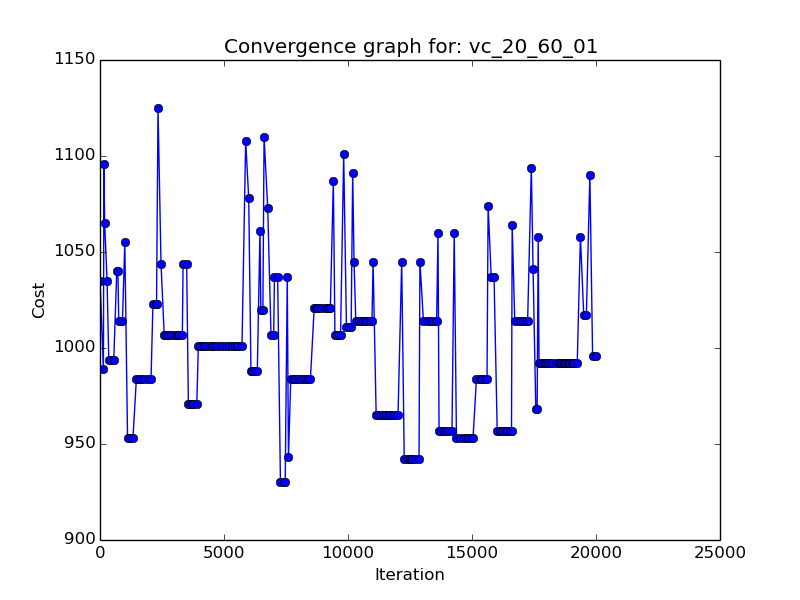
\includegraphics[width=\linewidth]{cg_1.png}
\end{minipage}%
\begin{minipage}{0.49\linewidth}
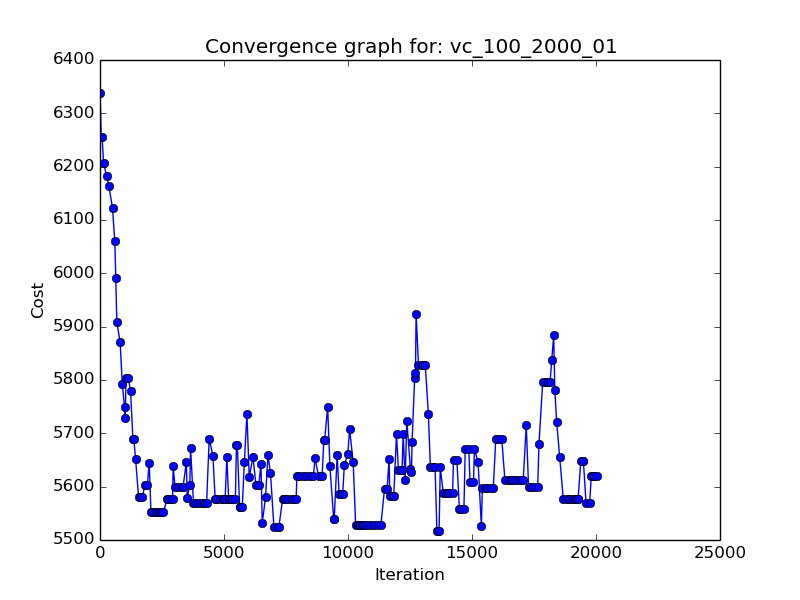
\includegraphics[width=\linewidth]{cg_2.png}
\end{minipage}
\begin{minipage}{0.49\linewidth}
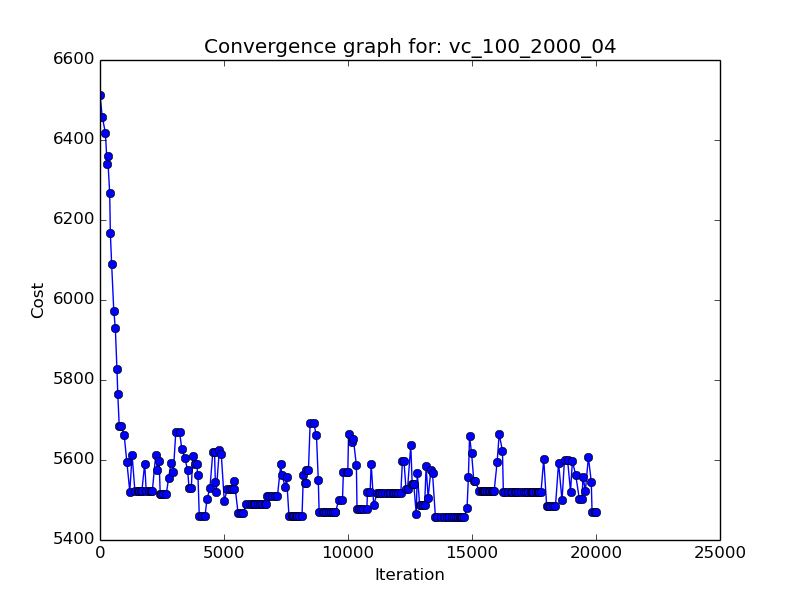
\includegraphics[width=\linewidth]{cg_3.png}
\end{minipage}
\begin{minipage}{0.49\linewidth}
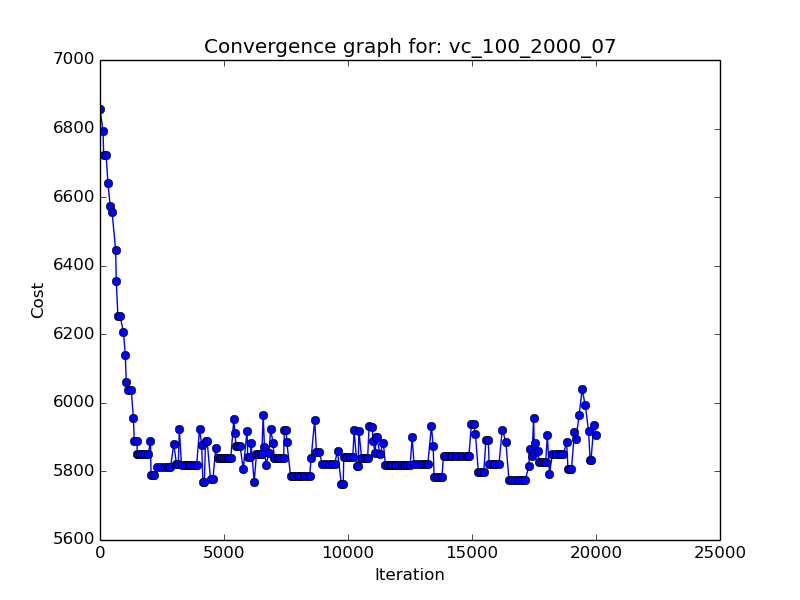
\includegraphics[width=\linewidth]{cg_4.png}
\end{minipage}
\begin{minipage}{0.49\linewidth}
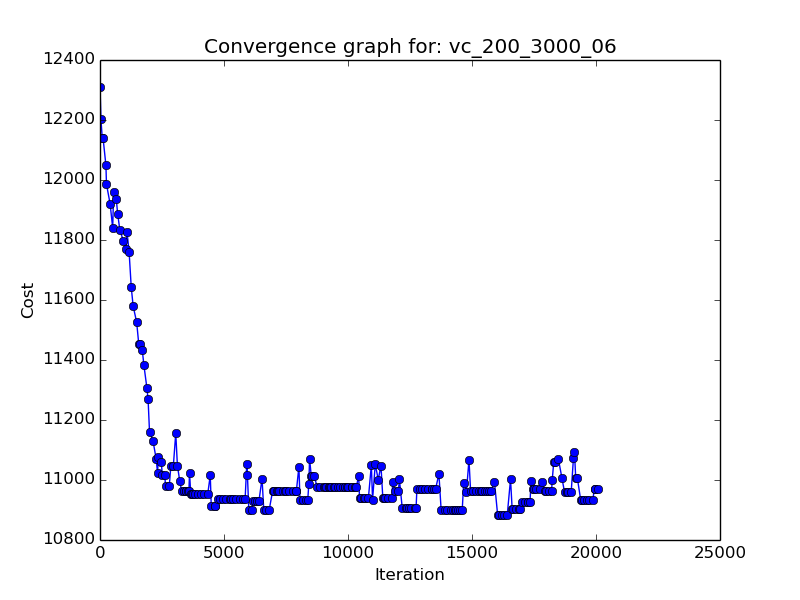
\includegraphics[width=\linewidth]{cg_5.png}
\end{minipage}
\begin{minipage}{0.49\linewidth}
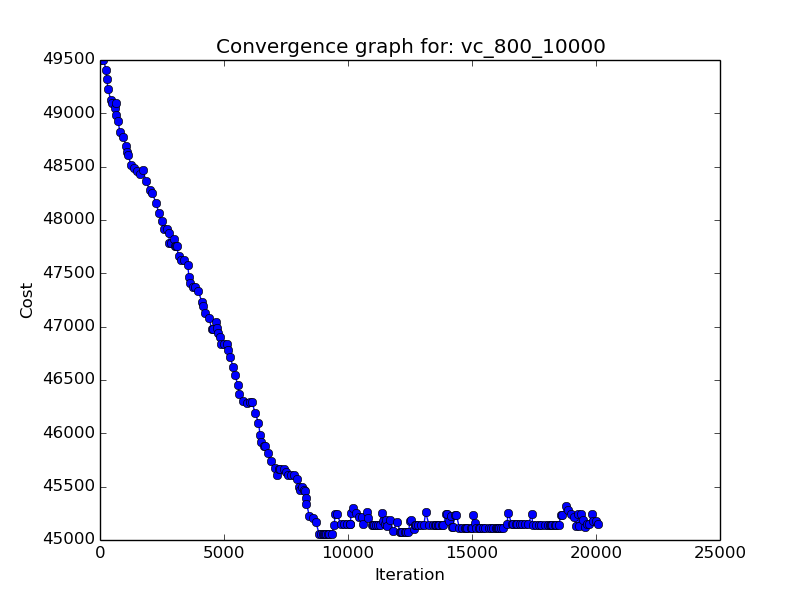
\includegraphics[width=\linewidth]{cg_6.png}
\end{minipage}
\captionof{figure}{Sample grafici di convergenza}
\end{center}


\pagebreak

Per quanto riguarda l'istanza LPI, i valori si riferiscono ad stata inserita una media su 10 run indipendenti dell'istanza.

\begin{table}[!ht]
    \centering
    \begin{tabular}{|l|l|l|}
    \hline
        instance & best solution & best solution iter \\ \hline
        vc\_800\_10000.txt & 45058 & 8841 \\ \hline
        vc\_25\_150\_10.txt & 1144 & 14059 \\ \hline
        vc\_25\_150\_09.txt & 1364 & 17960 \\ \hline
        vc\_25\_150\_08.txt & 1246 & 12629 \\ \hline
        vc\_25\_150\_07.txt & 1465 & 6028 \\ \hline
        vc\_25\_150\_06.txt & 1211 & 12562 \\ \hline
        vc\_25\_150\_05.txt & 1337 & 18720 \\ \hline
        vc\_25\_150\_04.txt & 1435 & 10635 \\ \hline
        vc\_25\_150\_03.txt & 1324 & 16454 \\ \hline
        vc\_25\_150\_02.txt & 1144 & 13880 \\ \hline
        vc\_25\_150\_01.txt & 1335 & 10656 \\ \hline
        vc\_20\_60\_10.txt & 960 & 2251 \\ \hline
        vc\_20\_60\_09.txt & 1149 & 3083 \\ \hline
        vc\_20\_60\_08.txt & 1113 & 2001 \\ \hline
        vc\_20\_60\_07.txt & 1033 & 1926 \\ \hline
        vc\_20\_60\_06.txt & 980 & 944 \\ \hline
        vc\_20\_60\_05.txt & 934 & 11274 \\ \hline
        vc\_20\_60\_04.txt & 819 & 7002 \\ \hline
        vc\_20\_60\_03.txt & 750 & 2788 \\ \hline
        vc\_20\_60\_02.txt & 1077 & 893 \\ \hline
        vc\_20\_60\_01.txt & 930 & 7276 \\ \hline
        vc\_20\_120\_10.txt & 1054 & 2723 \\ \hline
        vc\_20\_120\_09.txt & 1160 & 20093 \\ \hline
        vc\_20\_120\_08.txt & 1099 & 17086 \\ \hline
        vc\_20\_120\_07.txt & 945 & 2289 \\ \hline
        vc\_20\_120\_06.txt & 919 & 2064 \\ \hline
        vc\_20\_120\_05.txt & 939 & 18957 \\ \hline
        vc\_20\_120\_04.txt & 1031 & 3640 \\ \hline
        vc\_20\_120\_03.txt & 960 & 648 \\ \hline
        vc\_20\_120\_02.txt & 1028 & 19134 \\ \hline
        vc\_20\_120\_01.txt & 898 & 16987 \\ \hline
    \end{tabular}
\end{table}

\pagebreak

\begin{table}[!ht]
    \centering
    \begin{tabular}{|l|l|l|l|}
    \hline
        instance & best solution & best solution iter \\ \hline

        vc\_200\_750\_10.txt & 9506 & 5725 \\ \hline
        vc\_200\_750\_09.txt & 10194 & 12447 \\ \hline
        vc\_200\_750\_08.txt & 9977 & 10051 \\ \hline
        vc\_200\_750\_07.txt & 8962 & 19990 \\ \hline
        vc\_200\_750\_06.txt & 9401 & 18489 \\ \hline
        vc\_200\_750\_05.txt & 10469 & 16295 \\ \hline
        vc\_200\_750\_04.txt & 9585 & 18489 \\ \hline
        vc\_200\_750\_03.txt & 9967 & 18263 \\ \hline
        vc\_200\_750\_02.txt & 10122 & 18489 \\ \hline
        vc\_200\_750\_01.txt & 9897 & 18489 \\ \hline
        vc\_200\_3000\_10.txt & 11027 & 12843 \\ \hline
        vc\_200\_3000\_09.txt & 11412 & 16213 \\ \hline
        vc\_200\_3000\_08.txt & 11265 & 4097 \\ \hline
        vc\_200\_3000\_07.txt & 11290 & 11685 \\ \hline
        vc\_200\_3000\_06.txt & 10885 & 16032 \\ \hline
        vc\_200\_3000\_05.txt & 11193 & 6571 \\ \hline
        vc\_200\_3000\_04.txt & 12054 & 12688 \\ \hline
        vc\_200\_3000\_03.txt & 11298 & 10718 \\ \hline
        vc\_200\_3000\_02.txt & 10938 & 17094 \\ \hline
        vc\_200\_3000\_01.txt & 11015 & 19143 \\ \hline
        vc\_100\_500\_10.txt & 5234 & 15582 \\ \hline
        vc\_100\_500\_09.txt & 5202 & 15612 \\ \hline
        vc\_100\_500\_08.txt & 5194 & 16926 \\ \hline
        vc\_100\_500\_07.txt & 5584 & 7796 \\ \hline
        vc\_100\_500\_06.txt & 5478 & 10191 \\ \hline
        vc\_100\_500\_05.txt & 5476 & 8037 \\ \hline
        vc\_100\_500\_04.txt & 5309 & 13155 \\ \hline
        vc\_100\_500\_03.txt & 5101 & 13155 \\ \hline
        vc\_100\_500\_02.txt & 5531 & 18855 \\ \hline
        vc\_100\_500\_01.txt & 5299 & 12145 \\ \hline
        vc\_100\_2000\_10.txt & 5676 & 16365 \\ \hline
        vc\_100\_2000\_09.txt & 5351 & 2727 \\ \hline
        vc\_100\_2000\_08.txt & 5633 & 14463 \\ \hline
        vc\_100\_2000\_07.txt & 5764 & 9729 \\ \hline
        vc\_100\_2000\_06.txt & 5394 & 15683 \\ \hline
        vc\_100\_2000\_05.txt & 5671 & 16801 \\ \hline
        vc\_100\_2000\_04.txt & 5458 & 13524 \\ \hline
        vc\_100\_2000\_03.txt & 5255 & 11275 \\ \hline
        vc\_100\_2000\_02.txt & 5388 & 2967 \\ \hline
        vc\_100\_2000\_01.txt & 5517 & 13586 \\ \hline

    \end{tabular}
\end{table}

\pagebreak

Una delle difficoltà più grandi trovate durante l'implementazione è stato quello di determinare se i criteri di scelta fossero effettivamente robusti o no. Sarebbe interessante proseguire con lo studio del problema continuando sui seguenti punti:

\begin{itemize}
    \item{implementare altri criteri per la selezione del nodo;}
    \item{implementazione e studio di altri criteri di accettazione;}
    \item{perfezionare l'algoritmo su istanze piccole;}
    \item{testare implementazione con altre soluzioni di partenza.}
\end{itemize}

\pagebreak

\begin{thebibliography}{6}

\bibitem{1} \href{https://www.researchgate.net/publication/242463011_An_Effective_Algorithm_for_Minimum_Weighted_Vertex_Cover_problem}{An Effective Algorithm for Minimum Weighted Vertex Cover Problem}
\bibitem{2} \href{https://www.cs.umd.edu/class/fall2018/cmsc858E/pdfs/651/vc.pdf} {Two approximation algorithm for Vertex Cover} 
\bibitem{3} \href{https://ieeexplore.ieee.org/abstract/document/7550782}{A fast heuristic for the minimum weight vertex cover problem}
\bibitem{4} \href{https://www.researchgate.net/publication/242463011_An_Effective_Algorithm_for_Minimum_Weighted_Vertex_Cover_problem}{An Effective Algorithm for Minimum Weighted Vertex Cover Problem}
\bibitem{5} \href{https://www.sciencedirect.com/science/article/abs/pii/S0377221720300278}{A memory-based iterated local search algorithm for the multi-depot open vehicle routing problem}
\bibitem{6} \href{https://ieeexplore.ieee.org/document/7550782}{A fast euristic for the minimum weight vertex cover problem}

\end{thebibliography}


\pagebreak
%--/Paper--

\end{document}
